\documentclass[10pt]{beamer}

\ifx\pdfoutput\undefined
% we are running LaTeX, not pdflatex
\usepackage{graphicx}
\else
% we are running pdflatex, so convert .eps files to .pdf
\usepackage{graphicx}
\usepackage{epstopdf}
\usepackage[level]{datetime}
\usepackage{enumerate}
\usepackage{amsmath}
\usepackage{amssymb}
\fi

\newdateformat{ukdate}{\ordinaldate{\THEDAY} \monthname[\THEMONTH] \THEYEAR}%������

%--------------------------------------------------------
% NOTE: 1) This is an UNOFFICIAL LaTeX beamer style for
%           Beihang University.
%       2) This is not exactly a beamer style, rather
%           it contains two LaTeX files to be inserted
%           in the slides' source file.
%       3) These files are based on Edward Hartley's work
%   <http://www-control.eng.cam.ac.uk/Main/EdwardHartley>
%       4) Complaints or suggestions are always welcome.
%
% Xiaoke Yang (das.xiaoke@hotmail.com)
% Wed 15 Jun 11:02:17 CST 2016
%--------------------------------------------------------


%--------------------------------------------------------
% Set up the Beihang University Colours for use with
% xcolor
%--------------------------------------------------------

% Blue palette
\definecolor{coreBlue}{rgb}{0 0.2745 0.4313} %#254aa5


%--------------------------------------------------------
% NOTE: 1) This is an UNOFFICIAL LaTeX beamer style for
%           Beihang University.
%       2) This is not exactly a beamer style, rather
%           it contains two LaTeX files to be inserted
%           in the slides' source file.
%       3) These files are based on Edward Hartley's work
%   <http://www-control.eng.cam.ac.uk/Main/EdwardHartley>
%       4) Complaints or suggestions are always welcome.
%
% Xiaoke Yang (das.xiaoke@hotmail.com)
% Wed 15 Jun 11:02:17 CST 2016
%--------------------------------------------------------

%--------------------------------------------------------
% Require tikz to do some text positioning
%--------------------------------------------------------
\usepackage{tikz}

%--------------------------------------------------------
% Use Helvetica rather than Computer Modern Sans Serif
% Comment this out if you prefer Computer Modern
%\usepackage{times}
%--------------------------------------------------------
%\usepackage{helvet}

%--------------------------------------------------------
% If you wish to use Arial, and have the winfonts package
% correctly installed uncomment the following to make the
% default sans serif font Arial
%--------------------------------------------------------
%\usepackage{winfonts}
%\usepackage[T1]{fontenc}
%\renewcommand{\sfdefault}{arial}
%--------------------------------------------------------

%--------------------------------------------------------
% Get rid of the navigation bar
%--------------------------------------------------------
\beamertemplatenavigationsymbolsempty

%--------------------------------------------------------
% Set the files corresponding to the University crests
% here
%--------------------------------------------------------
% Crest with blue text
\newcommand{\beihangcrestblack}{beihangbeamerstyle/lable.pdf}

% Crest with white text
\newcommand{\beihangcrestwhite}{beihangbeamerstyle/lable2.pdf}
%--------------------------------------------------------

%--------------------------------------------------------
% Define how the page counter will be displayed on slides
%--------------------------------------------------------
\newcommand{\footlinepagecounter}%
	{\insertframenumber{}/\inserttotalframenumber}
%--------------------------------------------------------

%--------------------------------------------------------
% Set up some lengths
%--------------------------------------------------------
% A paper width for the footline
\newlength{\halfpaperwidth}

% The left margin
\newlength{\headingleftmargin}
% Paper width minus margins
\newlength{\headingwidthminusmargins}
% Height of the heading block
\newlength{\headingheight}
% Height of the footer block
\newlength{\footerheight}

% The height for the titlepageheader in the title page
\newlength{\titlepageheaderheight}
% The height for the footer in the title page
\newlength{\titlepagefooterheight}
% The height for the main title block
\newlength{\titlepagemaintitleblockheight}
% The height for the subtitle block
\newlength{\titlepagesubtitleblockheight}
% The height for the name and date block
\newlength{\titlepagenamedateblockheight}
% The height for the institution block
%\newlength{\titlepageinstitutionheight}

% The lengths for spacing between name and date
\newlength{\titlepagespaceundername}
\newlength{\titlepagespaceunderdate}

% The length for the light blue thin bar


\setlength{\headingleftmargin}{0.05573\paperwidth}
\setlength{\headingwidthminusmargins}{\paperwidth}
\addtolength{\headingwidthminusmargins}{-\headingleftmargin}
\setlength{\headingheight}{0.1459\paperheight}
\setlength{\footerheight}{0.09017\paperheight}

\setlength{\titlepageheaderheight}{0.2361\paperheight}
\setlength{\titlepagefooterheight}{0.1459\paperheight}
\setlength{\titlepagemaintitleblockheight}{0.2361\paperheight}
\setlength{\titlepagesubtitleblockheight}{0.1459\paperheight}
\setlength{\titlepagenamedateblockheight}{0.2361\paperheight}
%\setlength{\titlepageinstitutionheight}{0.95cm}

\setlength{\titlepagespaceundername}{16pt}
\setlength{\titlepagespaceunderdate}{8pt}

%--------------------------------------------------------

%--------------------------------------------------------
% Set up the Beihang University blue scheme for use
% with beamer
%--------------------------------------------------------

% Define colour names
\setbeamercolor{coreBlue}{bg=coreBlue, fg=white}

% Set element colours
\setbeamercolor{subtitle}{fg=white}
\setbeamercolor{titlepageheader}{bg=white,fg=black}
\setbeamercolor{titlepagefooter}{bg=white,fg=black}
\setbeamercolor{block title}{bg=white, fg=coreBlue}
\setbeamercolor{structure}{bg=white, fg=coreBlue}
% \setbeamercolor{alerted text}{fg=darkOrange}


%--------------------------------------------------------
% Set font sizes
%--------------------------------------------------------
\setbeamerfont{frametitle}{size=\large,series=\bfseries}
\setbeamerfont{title}{size=\large,series=\bfseries}
\setbeamerfont{author}{size=\normalsize}
\setbeamerfont{date}{size=\scriptsize}
\setbeamerfont{subtitle}{size=\footnotesize,series=\bfseries}
\setbeamerfont{block title}{size=\normalsize,series=\bfseries}
\setbeamerfont{structure}{size=\normalsize,series=\bfseries}

\setbeamertemplate{itemize item}{\scriptsize\raise1.25pt\hbox{\textbullet}}
\setbeamertemplate{itemize subitem}{\scriptsize\raise1.25pt\hbox{\textbullet}}
\setbeamertemplate{itemize subsubitem}{\scriptsize\raise1.25pt\hbox{\textbullet}}


%-----------------------------------------------------
% Define frame title drawing
%-----------------------------------------------------
\setbeamertemplate{frametitle}
{%
  \nointerlineskip
  \begin{beamercolorbox}[wd=\paperwidth,leftskip=\headingleftmargin]{coreBlue}
    \vskip1pt%
    \tikz{\node[minimum height=\headingheight, inner sep=0cm, text width= \headingwidthminusmargins, text badly ragged]{\usebeamerfont{frametitle}\insertframetitle\\\normalsize\it\insertframesubtitle};}
  \end{beamercolorbox}%
}

%-----------------------------------------------------
% Define footline drawing
%-----------------------------------------------------
\setbeamertemplate{footline}
{%
 \setlength{\halfpaperwidth}{0.5\paperwidth}
 \addtolength{\halfpaperwidth}{1pt}
 \leavevmode
 \begin{beamercolorbox}[sep=0pt,wd=\halfpaperwidth, leftskip=\headingleftmargin,right]{coreBlue}
 \tikz{\node[minimum height=\footerheight, inner sep=0cm]{\footlinepagecounter};}%
 \end{beamercolorbox}
 \hskip-1.5pt%
 \begin{beamercolorbox}[sep=0pt,wd=\halfpaperwidth, leftskip=\headingleftmargin, right,rightskip=\headingleftmargin]{coreBlue}
 \tikz{\node[minimum height=\footerheight, inner sep=0cm]{\includegraphics[width=0.25\paperwidth]{\beihangcrestwhite}};}%
 \end{beamercolorbox}%
}


%-----------------------------------------------------
% Define BEIHANG title page
%-----------------------------------------------------
\setbeamertemplate{title page}
{%
\begin{beamercolorbox}[sep=0cm,right,wd=\paperwidth,ht=\titlepageheaderheight,rightskip=\headingleftmargin]{titlepageheader}
\includegraphics[width=0.3820\paperwidth]{\beihangcrestblack}
\vskip0.2361\titlepageheaderheight
\end{beamercolorbox}
\begin{beamercolorbox}[left,leftskip=\headingleftmargin,wd=\paperwidth,ht=\titlepagemaintitleblockheight]{coreBlue}
\tikz{\node[inner sep=0cm, text width=\paperwidth, minimum height=\titlepagemaintitleblockheight,text badly ragged]{\usebeamerfont{title}\inserttitle};}%
\end{beamercolorbox}%
\nointerlineskip%
\vskip-1pt%
\begin{beamercolorbox}[left,leftskip=\headingleftmargin,wd=\paperwidth,ht=\titlepagesubtitleblockheight]{coreBlue}
\tikz{\node[inner sep=0cm, text width=\paperwidth, minimum height=\titlepagesubtitleblockheight, text badly ragged]{\usebeamerfont{subtitle}\usebeamercolor[fg]{subtitle}\insertsubtitle};}%
\end{beamercolorbox}%
\nointerlineskip%
\vskip-1pt%
\begin{beamercolorbox}[left,leftskip=\headingleftmargin,wd=\paperwidth,ht=\titlepagenamedateblockheight]{coreBlue}
      \usebeamerfont{author}\insertauthor\\
      \vskip\titlepagespaceundername%
      \usebeamerfont{date}\insertdate
      \vskip\titlepagespaceunderdate%
    \end{beamercolorbox}%
\begin{beamercolorbox}[left,leftskip=\headingleftmargin,wd=\paperwidth,ht=\titlepagefooterheight]{titlepagefooter}
\end{beamercolorbox}
}


\title{Spiking Neuron Model and Python Implement}
\author{Yan Zhou\\
Northeastern University (\texttt{zhouy@mail.neu.edu.cn})}
\date{Seminar, Shenyang, \ukdate\today}


\begin{document}
%----------------------------------------------------------------------
% Title frame
\begin{frame}[plain]
\maketitle
\end{frame}

%----------------------------------------------------------------------
% Outline frame
% PLEASE RUN pdflatex TWICE
\begin{frame}
\frametitle{Outline}
\tableofcontents
\end{frame}
%%=====================================================================
% Section I
\section{Neuronal Coding}
%----------------------------------------------------------------------
% Content frame
\begin{frame}\frametitle{Neuronal Coding}
%\framesubtitle{From the stimulus to Response}
\begin{block}{Introduction}
\begin{itemize}
\item Traditionally it has been thought that most, if not all, of the relevant information was contained in the mean firing rate of the neuron. Neuronal coding is a way of convert the pulses to analog values.
\item The relation between the measured firing frequency $v$ and the applied input current $I_0$ is sometimes called the {\color{red}{frequency-current curve}} of the neuron.
\item In models, we formalize the relation between firing frequency (rate) and input current and write $v = g(I_0)$. We refer to $g$ as the neuronal gain function or transfer function\cite{RN85}.
\item For instance, the quantity of electric charge $\varDelta tI_0=\int^{t+\Delta t}_t \sum_i e(\tau-t_i)\,d\tau$, and the firing rate satisfy $\varDelta tv=\int^{t+\Delta t}_t \sum_i \delta(\tau-t_i)\,d\tau$.
\end{itemize}
\end{block}
\end{frame}
%\pause
%----------------------------------------------------------------------
\begin{frame}
\begin{block}{Rate Codes}\frametitle{Neuronal Coding}
\begin{itemize} 
\item Average over time.
\item Average over several repetitions of the experiment.
\item Average over a population of neurons.
\end{itemize}
\end{block}
%\begin{block}{Another block}
%This block appears after a pause. Simply delete the \texttt{\textbackslash pause} command if this animation is not needed. Add the pause command whenever a pause is needed.
%\end{block}
\end{frame}
%----------------------------------------------------------------------
\begin{frame}\frametitle{Neuronal Coding}
\begin{block}{Rate as a Spike Count (Average over Time)}
\begin{equation}
\label{AOTe}
v=\frac{n_{sp}(T)}{T} = \frac {\int^T_0 \sum^{n_{sp}}_{i=1}\delta(\tau-t_i)d\tau}{T}
\end{equation}
\end{block}
\begin{figure}[htb]
\centering
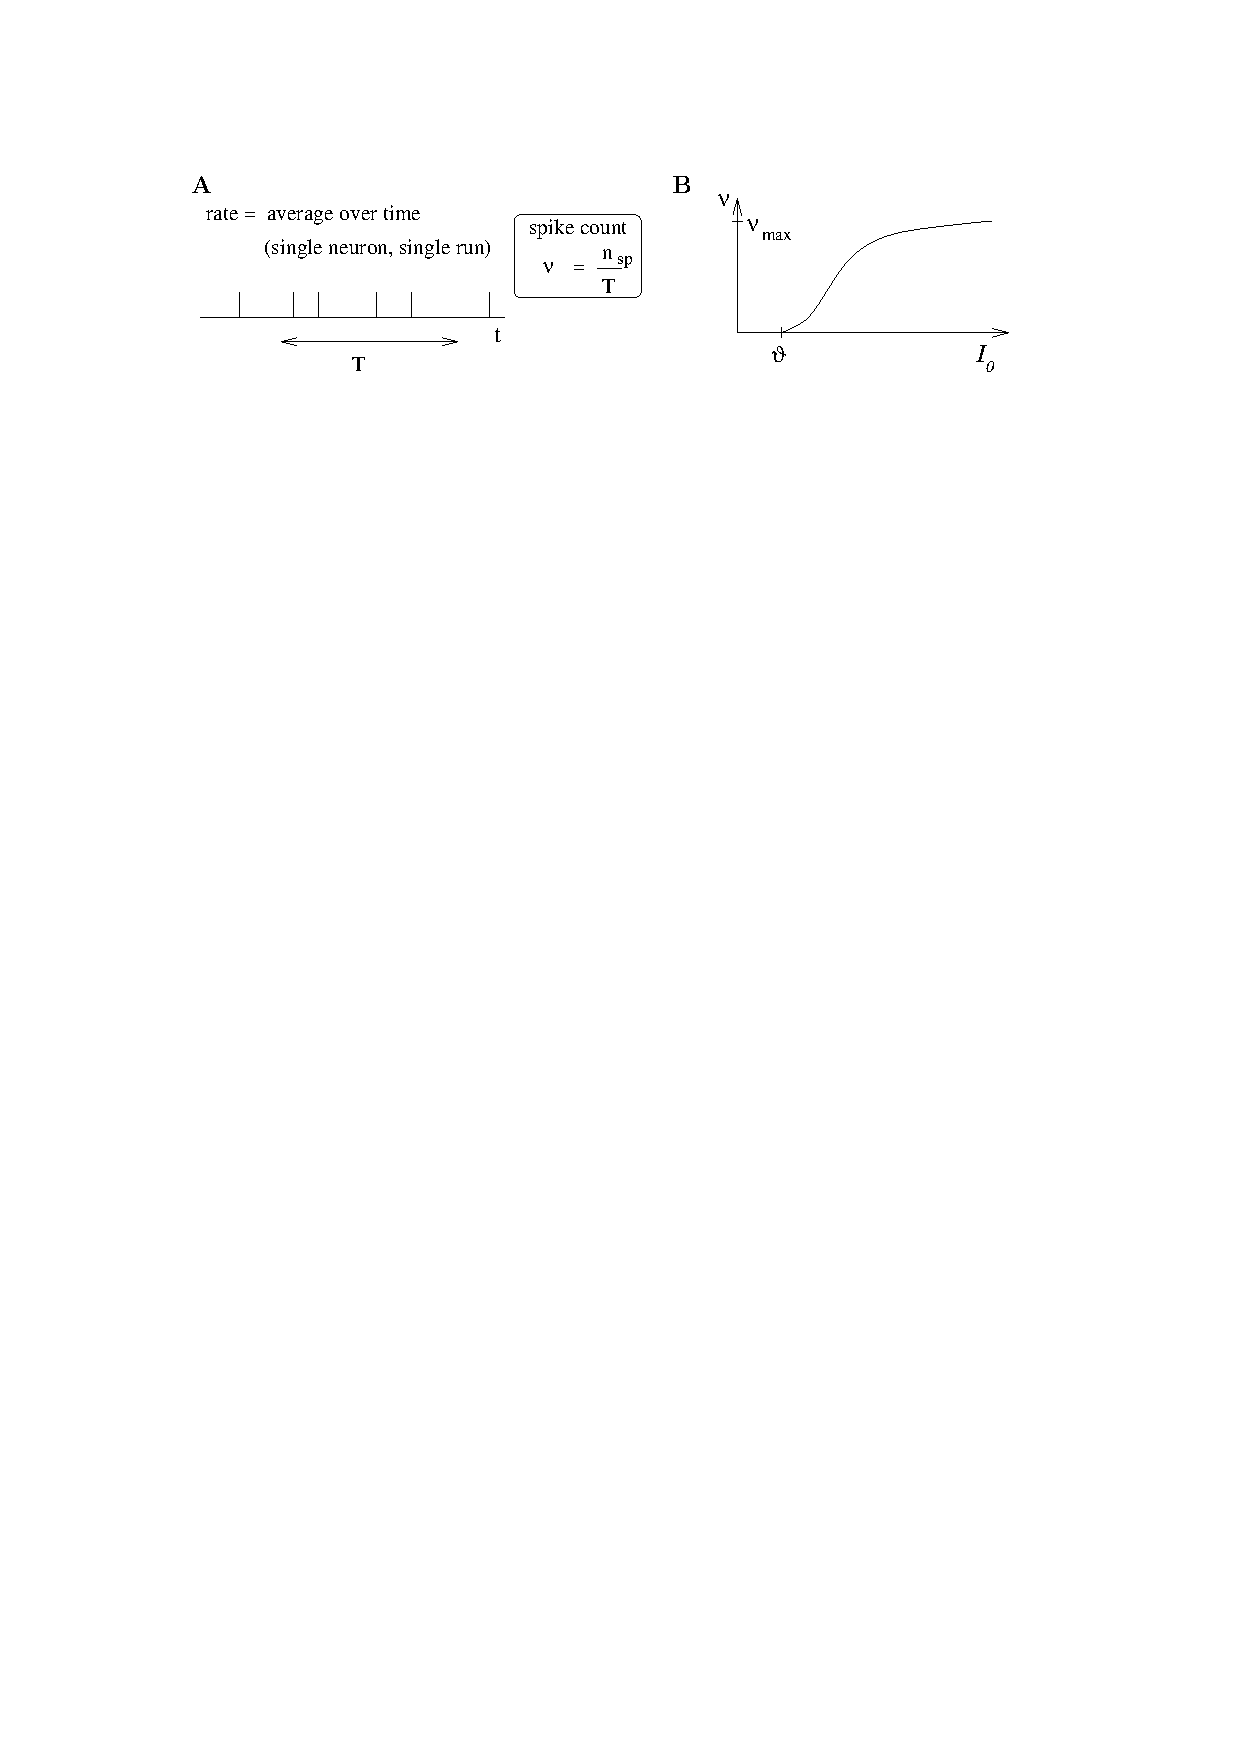
\includegraphics[width=0.9\linewidth]{image/1.pdf}
\caption{A. Definition of the mean firing rate via a temporal average. B. Gain function, schematic. The output rate $v$ is given as a function of the total input $I_0$.}
\label{AOT}
\end{figure}
\end{frame}
%----------------------------------------------------------------------
\begin{frame}\frametitle{Neuronal Coding}
\begin{block}{Rate as a Spike Density (Average over Several Runs)}
\begin{equation}
\label{AOSe}
v=\frac {1}{\Delta t} \frac{n_{k}(t;t+\Delta t)}{K}
\end{equation}
\end{block}
\begin{figure}[htb]
\centering
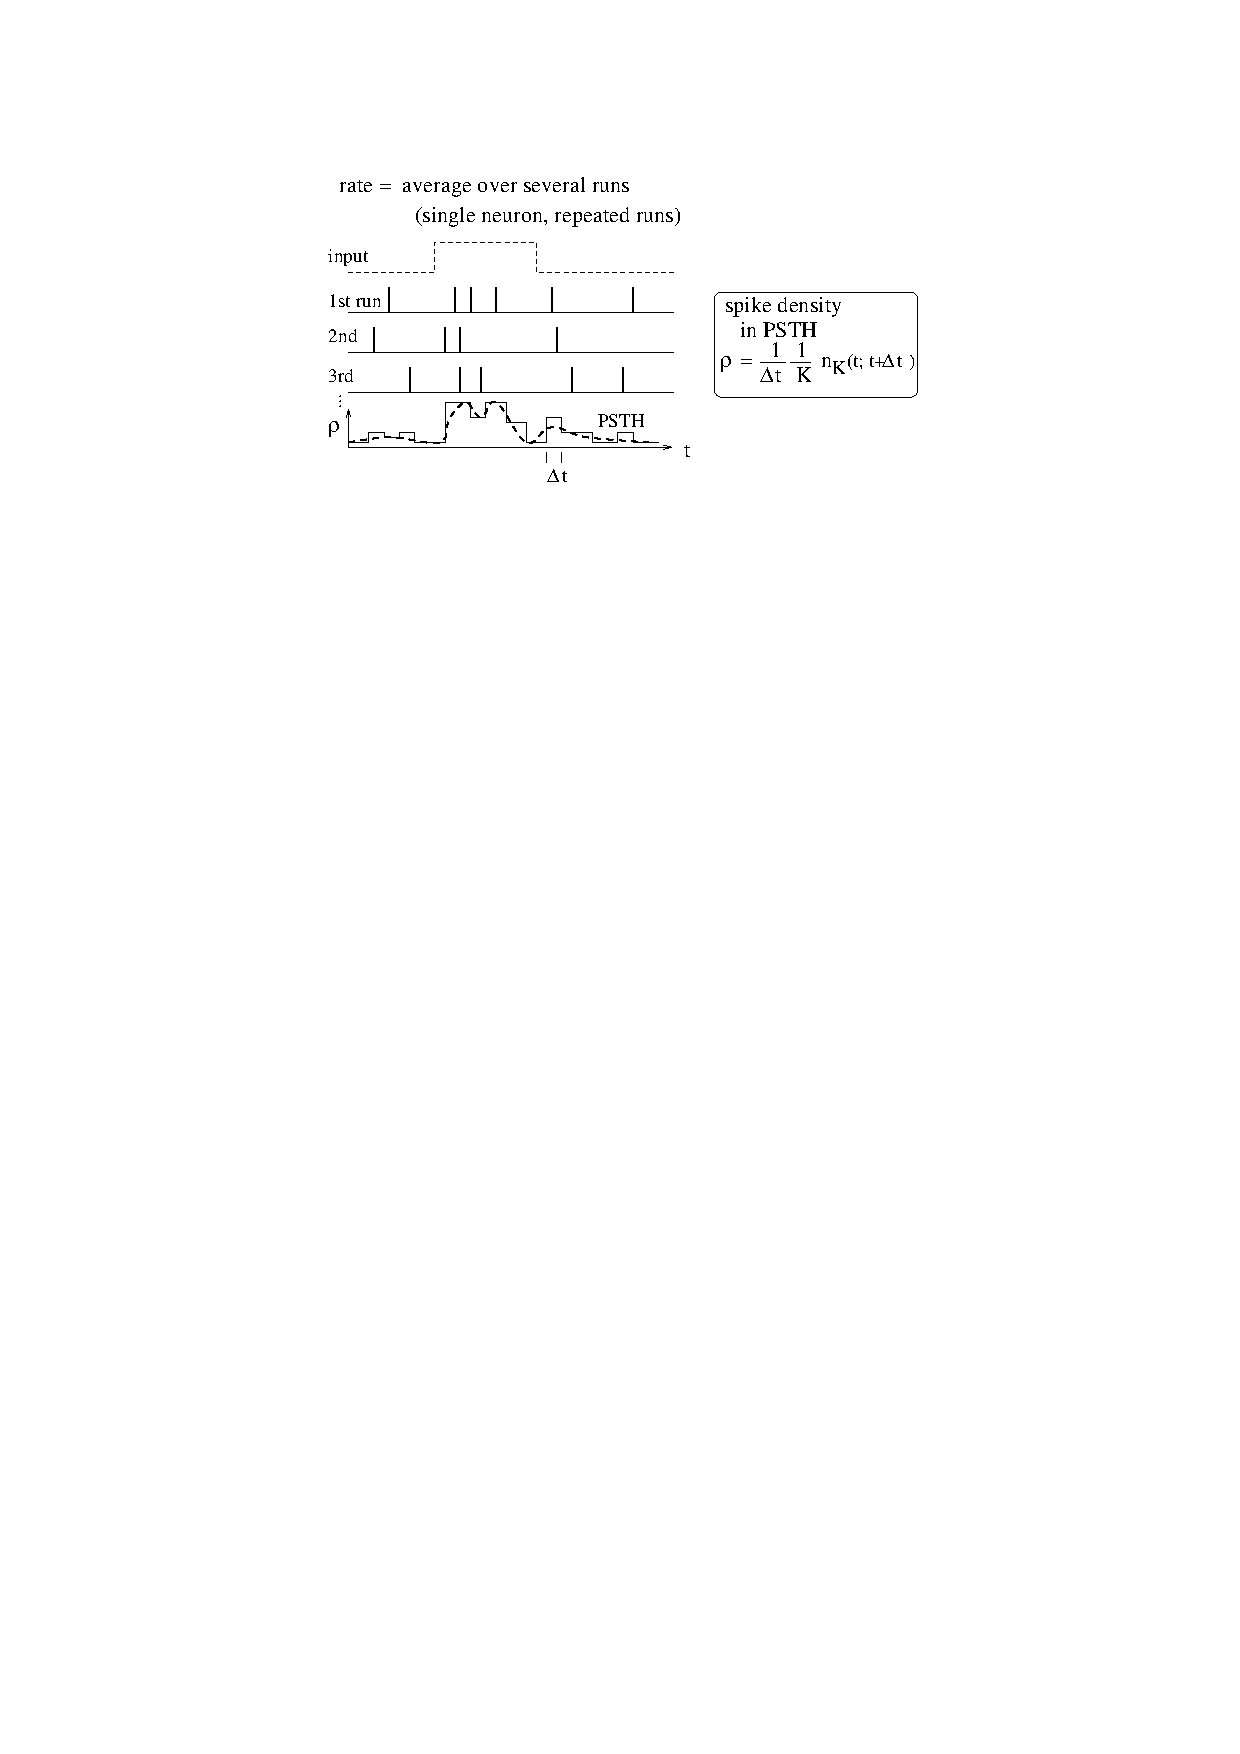
\includegraphics[width=0.6\linewidth]{image/2.pdf}
\caption{Definition of the spike density in the Peri-Stimulus-Time Histogram(PSTH) as an average over several runs of the experiment.}
\label{AOS}
\end{figure}
\end{frame}

%----------------------------------------------------------------------
\begin{frame}\frametitle{Neuronal Coding}
\begin{block}{Rate as a Population Activity (Average over Several Neurons)}
\begin{equation}
\label{AOSNe}
v=\frac {1}{\Delta t} \frac{n_{act}(t;t+\Delta t)}{N} = \frac {1}{\Delta t}\frac{\int^{t+\Delta t}_t \sum_j\sum_f\delta(\tau-t_j^{(f)})d \tau}{N}
\end{equation}
\end{block}
\begin{figure}[htb]
\centering
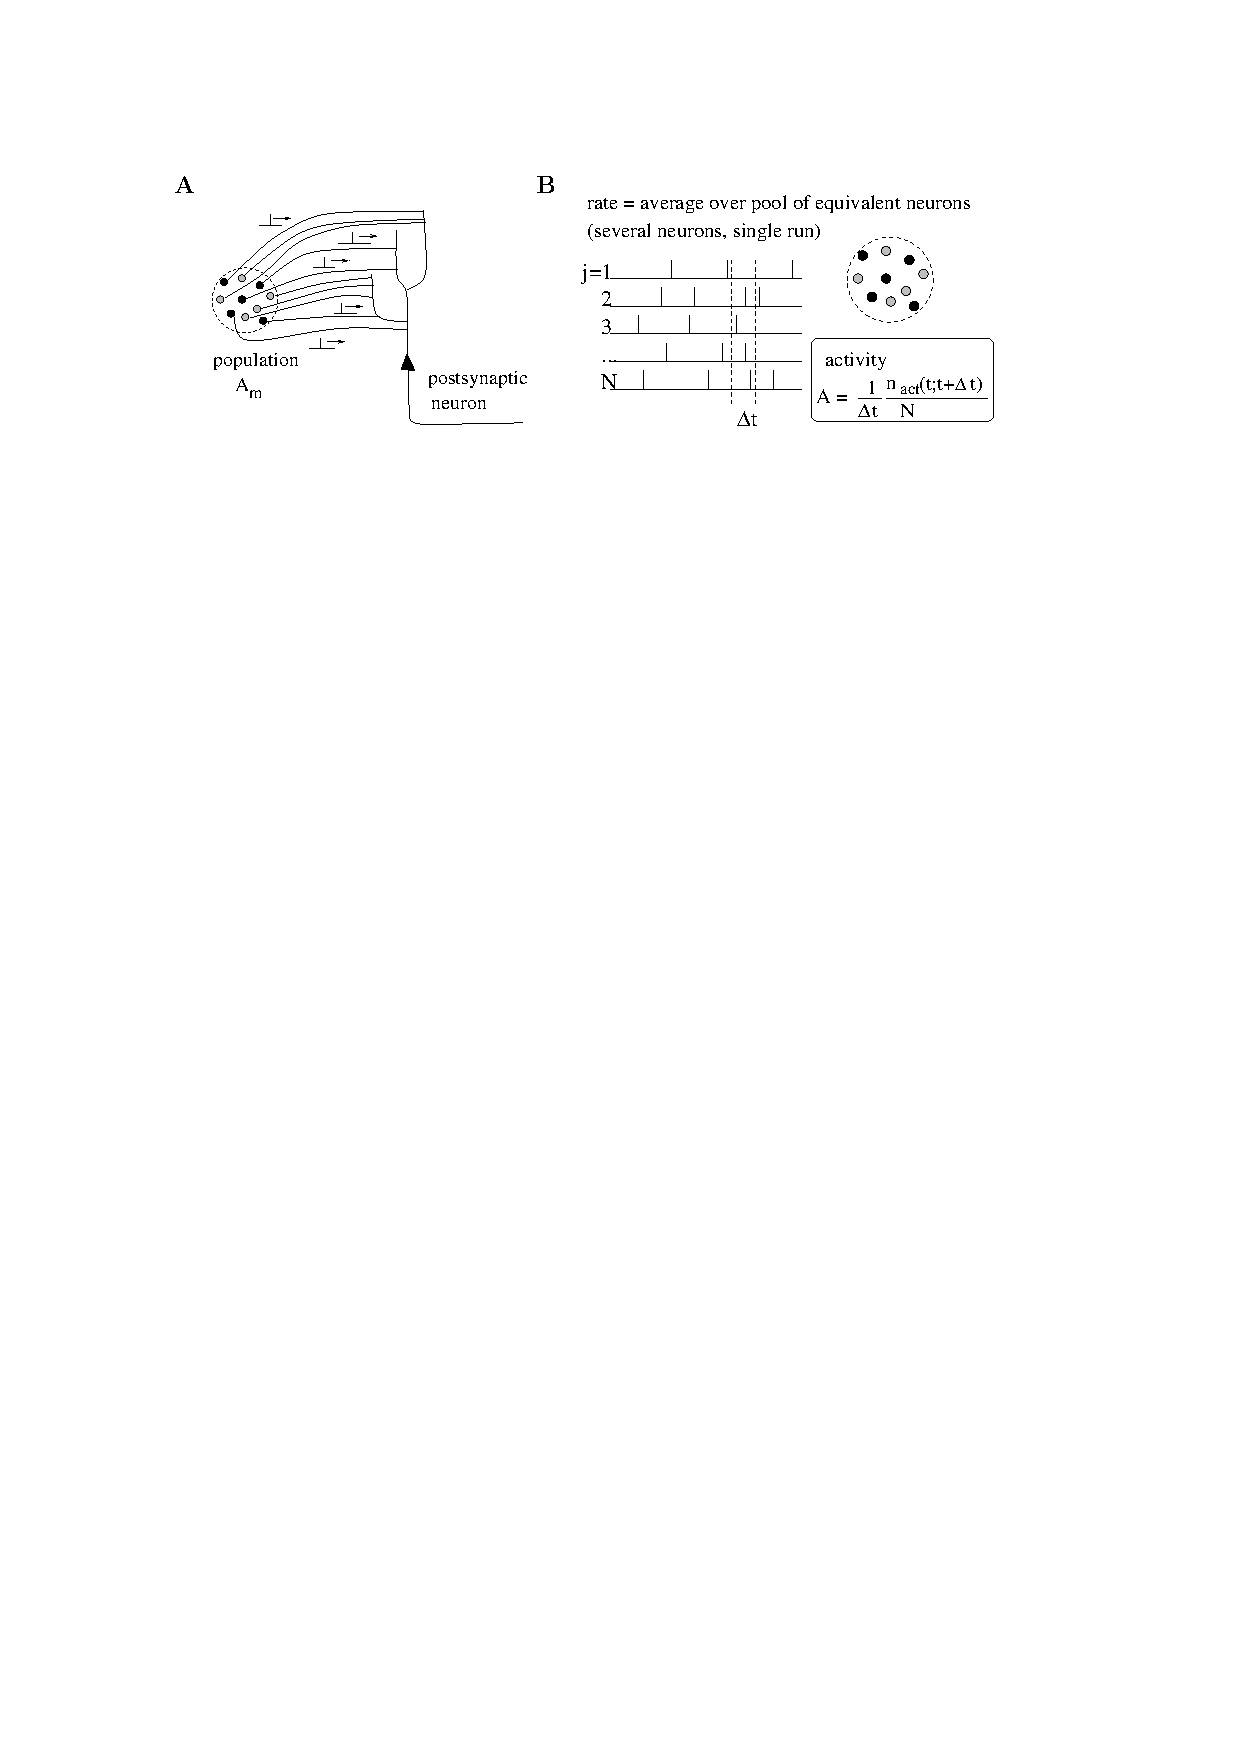
\includegraphics[width=0.8\linewidth]{image/3.pdf}
\caption{A. A postsynaptic neuron receives spike input from the population $m$ with activity $A_m$. B. The population activity is defined as the fraction of neurons that are active in a short interval $[t; t + \Delta t]$ divided by $\Delta t$.}
\label{AOSN}
\end{figure}
\end{frame}
%----------------------------------------------------------------------
\begin{frame}
\frametitle{More Detailed Methods of Neuronal Coding}
\begin{columns}
\begin{column}{0.5\textwidth}
\begin{figure}[htb]
\centering
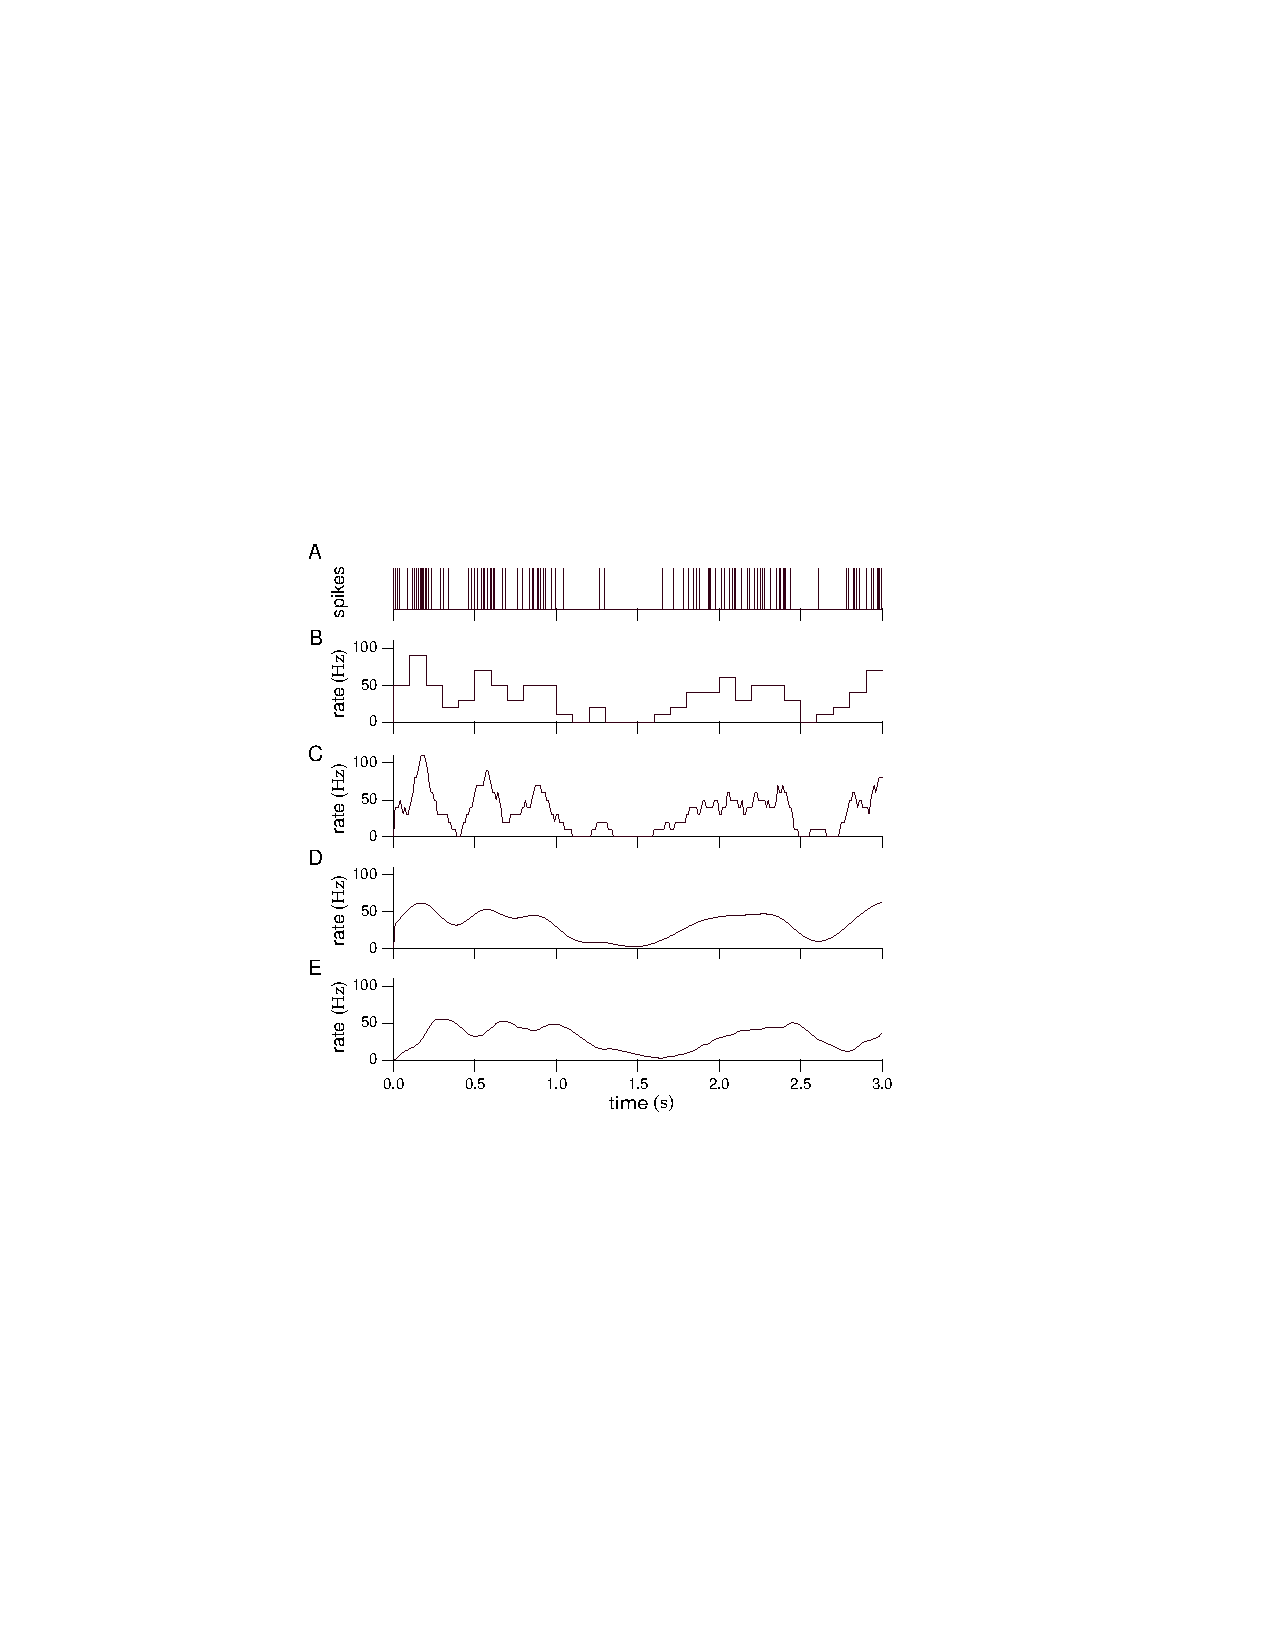
\includegraphics[width=1\linewidth]{image/4.pdf}
\caption{Firing rates approximated by different procedures\cite{RN113}.}
\label{A}
\end{figure}

\end{column}
\begin{column}{0.5\textwidth}
\begin{block}{Counting \& Convolution}
\alt<2>{
\begin{itemize}
\item $v_{approx}(t)=\sum^n_{i=1}w(t-t_i)=\int_{-\infty}^{+\infty} \sum^n_{i=1} d(\tau)w(\tau)\delta(t-\tau)$
\item $w(\tau) = \begin{cases} 1/\Delta t \quad if -\Delta t/2\geqslant t \ge \Delta t/2 \\0 \qquad otherwise.\end{cases}$
\item $w(\tau) = \frac {1}{\sqrt{2\pi}\sigma}exp(-\frac{\tau^2}{2\sigma^2})$.
\end{itemize}}
{\begin{enumerate}[(A)]
\item A spike train from a neuron.
\item Discrete time firing rate obtained by counting spikes 
\item Approximate firing rate determined by sliding a rectangular window function along the spike train. 
\item Approximate firing rate computed using a Gaussian window function. 
\item Approximate firing rate for an $\alpha$ function window.
\end{enumerate}}
%{\color{coreBlue}{This is the only ``Beihang colour'' I found. }} Other built-in colours can also be used, e.g. {\color{red}{red}}, {\color{orange}{orange}}, {\color{blue}{blue}}
%\vspace{9.5em}

\end{block}
\end{column}
\end{columns}
\end{frame}

%%=====================================================================
% Section II
\section{Formal Spiking Neuron Model}
%----------------------------------------------------------------------
\begin{frame}
\frametitle{\secname}
\begin{block}{Formal threshold models of neuronal firing}
Spikes are generated whenever the membrane potential $u$ crosses some threshold $\vartheta$ from below. The moment of threshold crossing defines the firing time $t(f)$.
\begin{equation}
\label{FSNM}
t^{(f)}: \quad u(t^{(f)})=\vartheta \quad and \quad \frac {du(t)}{dt}\big|_{t=t(f)}>0
\end{equation}
\end{block}
\end{frame}

%----------------------------------------------------------------------
\begin{frame}
\frametitle{\secname}
\begin{block}{Formal threshold models of neuronal firing}
\begin{itemize}
\item Integrate-and-fire model\cite{RN85}
    \begin{itemize}
    \item Leaky Integrate-and-Fire Model
    \item nonlinear Integrate-and-Fire Model
    \end{itemize}
\item Izhikevich Model\cite{RN96}
\end{itemize}
\end{block}
\end{frame}

%%=====================================================================
% Section III
\section{Spiking Neurons Design and Simulations}
%----------------------------------------------------------------------
\begin{frame}
\frametitle{Spiking Neurons Design and Simulations}
\begin{block}{Leaky Integrate-and-Fire Model}
\begin{figure}[htb]
\centering
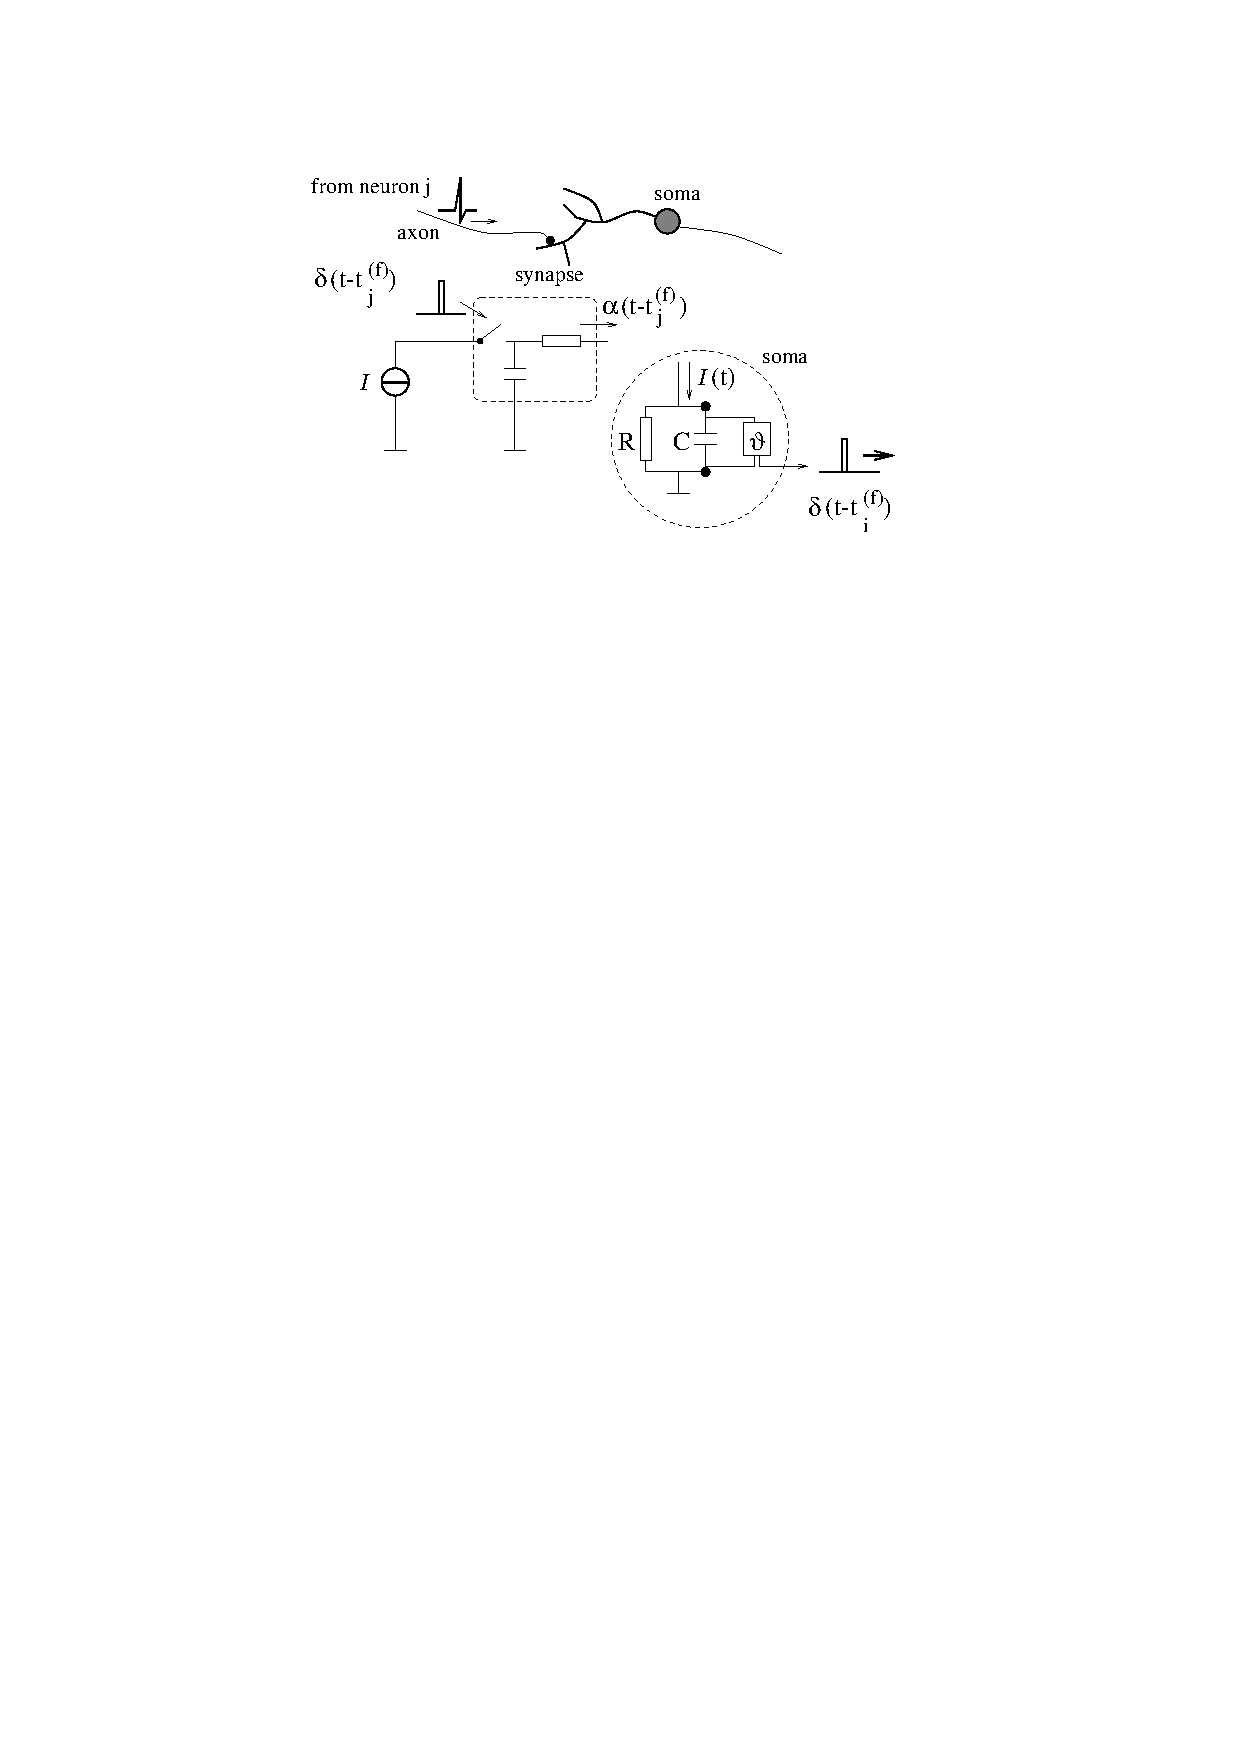
\includegraphics[width=0.6\linewidth]{image/5.pdf}
\caption{}
\label{LIF}
\end{figure}


\end{block}
\end{frame}

%%=====================================================================
% Section IV
\section{Bibliography}
%----------------------------------------------------------------------
\begin{frame}
\frametitle{Bibliography}
\bibliographystyle{plain}
\bibliography{reference}
\end{frame}
\end{document}

